\section{Control Plane Synthesis via ARCs} \label{sec:synthesis}
In this section, we describe preliminary ideas on how each phase of our synthesis 
approach can be implemented.
First, we briefly discuss how existing tools can be used to generate
policy-compliant paths (\secref{phase1}).
Second, we show how to generate ARCs that induce
the set of paths synthesized in the first phase (\secref{phase2}).
Third, we show how ARCs can be modified to deal with resilience (\secref{TODO}).
Finally, we show how to restart the process whenever one of the three phases fails (\secref{TODO}).

\subsection{From policies to paths} \label{sec:phase1}
The first phase of our approach produces a set of paths adhering to
different policies like reachability, service chaining, traffic engineering and isolation.
Synthesizing sets of paths---i.e., data planes---that adhere to a given set of policies
is already a hard problem, but a few practical approaches have been proposed.
The approach that is most similar to ours is the one used in Merlin~\cite{merlin}.
Given a set of waypoints, reachability, and bandwidth guarantee policies,
Merlin generates a mixed integer linear programming instance. 
A solution to this instance is a set of paths meeting the input policies.
Our prototype implementation uses a similar idea and,
since this part of the problem is not novel, we briefly provide the intuition behind our solution.
Given a set of policies we generate a set of constraints over the propositional theory of rationals 
and the solutions to these constraints are paths satisfying all the policies.
Our rich policy language requires complex Boolean reasoning that forces us to adopt propositional theories
in place of simple conjunctions of constraints.
In particular, policies like isolation and waypoints require disjunctive formulas.

%\loris{we will add more details if needed}


\subsection{From paths to ARCs} \label{sec:phase2}

The second phase of our approach takes as input the set of paths produced by the first phase
and produces an Abstract Representation of the Control Plane (ARC) that realizes the given set of paths.
First, we consider the problem of generating ARCs that
 forward packets based on shortest-paths---e.g., OSPF routing.
Then, we consider more complex forms of ARCs in which 
 additional mechanisms like route-filtering are allowed. 
 
\subsubsection{From paths to simplified ARCs} \label{sec:sarc}
The \emph{Simplified Abstract Representation of the Control Plane} (sARC) is a directed graph comprising switches as 
vertices and weighted edges corresponding to all links in the
topology. 
This is an ideal control plane supporting classic shortest path routing in which no links can be disabled. 

The problem of synthesizing 
a sARC that realizes an input set of paths reduces to a
variation of the so-called {\em inverse shortest path} problem~\cite{isp}. 
Assume we are given the following inputs: (1) a directed graph $T = (S, L)$ (the network topology), 
(2) a set of endpoints $\Gamma \subseteq S\times S$
describing the sources and destinations of the input paths, and 
(3) a function $P: \Gamma \rightarrow 2^{L^*}$
that assigns to each pair of endpoints $(s,t) \in \Gamma$ 
a set of \emph{acyclic} paths, such that for every path $l_0\cdots l_n\in P(s,t)$,
$l_0=(s,s')$, for some $s'\in S$, and $l_n=(s'',t)$, for some $s''\in S$.\footnote{
We use $L^*$ the denote the set of all finite sequences over the set $L$.}
The 
\emph{sARC synthesis}
problem is to find rational weights for the edges in $L$ such that 
for each pair of endpoints $(s,t) \in \Gamma$, 
the paths in $P(s,t)$ are \emph{the} shortest paths from $s$ to $t$ 
in the graph. Notice, that there can be multiple shortest
paths of equal cost for multi-path support (e.g., for traffic engineering).

In sARC, packet forwarding is based on destination.
For a destination $d$, we call $\xi_d$ the directed
subgraph of $T$ obtained by only keeping the nodes and edges 
that are traversed by paths with destination $d$.
Since paths are acyclic, $\xi_d$ is a directed acyclic graph.
We use $\Omega=\{d\mid (\_,d)\in\Gamma\}$ to denote the 
set of all destinations and $\Delta=\{\xi_d\mid d\in \Omega\}$ to denote  
the set of all destination DAGs. 

We use  $sw_1\rightarrow sw_2$ to denote $(sw_1,sw_2)\in L$ and
$sw_1\rightarrow^* sw_2$ (resp. $sw_1\rightarrow^+ sw_2$) to denote 
that $sw_2$ is reachable from $sw_1$ by crossing zero (resp. one) or more links in $T$.
Similarly, we use $\rightarrow_{\xi_d}$ to denote the same relations in the destination DAGs.


\minisection{Distance Equations}
To solve the sARC synthesis problem, we generate a set of linear equations
to find the required edge weights. 
We use $E(sw_1, sw_2)$ to denote the weight of the edge $(sw_1,sw_2)\in L$
and 
$D(sw_1, sw_2)$ to denote the shortest distance from $sw_1$ to $sw_2$.
We add the equation $D(s,s) = 0$ for every $s\in S$ to denote that the distance
from a node to itself is $0$.
The
following equation guarantees that $D(s,t)$ is not greater than 
the actual shortest distance from $s$ to $t$.
\begin{multline} \label{eq:dist}
\forall s, t, sw. (s \rightarrow sw \rightarrow^* t).\\
D(s, t) \leq E(s, sw) + D(sw, t)
\end{multline}

For each destination DAG $\xi_d\in\Delta$, we add equations to ensure 
that the input paths with destination $d$ are indeed the shortest ones.
 If a path
is the shortest path between its endpoints, then every 
subpath of the path has to be the shortest between its endpoints
as well (otherwise the complete path would not be the shortest).

 \begin{figure}[h!] 
 	\centering
 	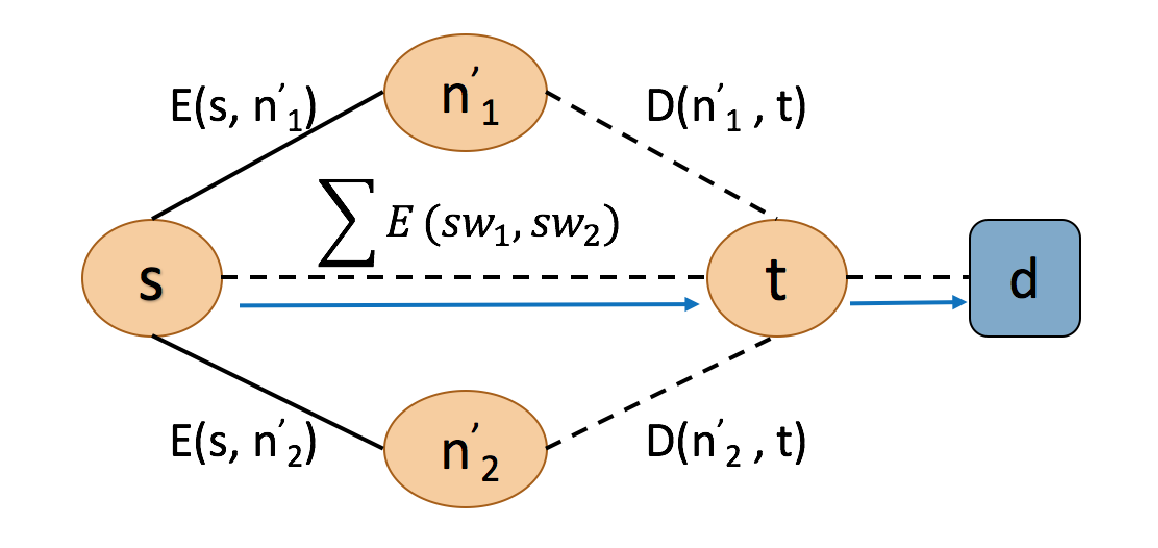
\includegraphics[width=0.75\columnwidth]{figures/distanceEquation.eps}
 	\caption{An example illustration of the distance equations for shortest path forwarding.
 		The pointed arrows represent the path in DAG of destination $d$, and the
 		dotted line represents 1 or more edges. 
 	} \label{fig:disteq}
 \end{figure}
Consider a DAG $\xi_d$ for destination $d$. We define two neighbour
functions: $N_T(s)$ denotes the set of neighbours of switch $s$ 
in the input graph $T$, and $N_{\xi_d}(s)$ denote the set of
neighbours of switch $s$ in the destination DAG $\xi_d$. 
Given a destination $d\in \Omega$,
we use the following equations to ensure that, given two nodes $s$ and $t$ in
$\xi_d$, 
the set of paths from $s$ to $t$ in $\xi_d$ are
exactly
\emph{the} shortest paths from $s$ to $t$ in $T$ (\Cref{fig:disteq} illustrates 
an example).
Let $s,t$ be two nodes in $\xi_d$ and let  $Paths_{\xi_d}(s,t)$ be the set of paths from $s$ to $t$ in $\xi_d$.
\begin{multline} \label{eq:uniq1}
		\forall l_0\cdots l_n\in Paths_{\xi_d}(s,t).
		\forall n' \in N(s) \setminus N_{\xi_d}(s). \\
		E(s, n') + D(n', t) > \sum_{\mathclap{\substack{l_i=(s_i,t_i)}}} 
		E(s_i, t_i) 
\end{multline}
\begin{multline} \label{eq:uniq2}
		\forall l_0\cdots l_n\in Paths_{\xi_d}(s,t).
		\forall n' \in N_{\xi_d}(s). n' \not\rightarrow^+_{\xi_d} t.  \\
		E(s, n') + D(n', t) > \sum_{\mathclap{\substack{l_i=(s_i,t_i)}}} 
		E(s_i, t_i) 
\end{multline}
\begin{multline} \label{eq:uniq3}
		\forall l_0\cdots l_n, l_0'\cdots l_n'\in Paths_{\xi_d}(s,t).\\
		\sum_{\mathclap{\substack{l_i=(s_i,t_i)}}} 
		E(s_i, t_i)  =\sum_{\mathclap{\substack{l_i'=(s_i',t_i')}}} 
		E(s_i', t_i') 
\end{multline}
Equation~\ref{eq:uniq1} guarantees that 
the sum of the weights belonging to a path from $s$ to $t$ in $\xi_d$ is smaller than 
any path that goes to $t$ via a node $n'$ that is a neighbour of $s$ in $T$ but not in $\xi_d$.
Equation~\ref{eq:uniq2} guarantees that
the sum of the weights belonging to a path from $s$ to $t$ in $\xi_d$ is smaller than 
any path that goes to $t$ via a node $n'$ that is a neighbour of $s$ in $\xi_d$ but such that
$t$ is not reachable from $n'$ in $\xi_d$.
Finally, Equation~\ref{eq:uniq2} guarantees that all the paths from $s$ to $t$ in $\xi_d$ have the same weight.

% If the path $n' \rightarrow^* t$ 
% is not in any DAG completely, then
% $D(n',t)$ can be smaller than the actual shortest distance by the
% semantics of \Cref{eq:dist} (as
% $D(n',t)$ is not equal to any quantity by \Cref{eq:shortest}).
% However, since $D(n',t)$ is on the RHS of the equations in \Cref{eq:uniq},
% the equations will ensure that the path $s\rightarrow n \rightarrow^* t$
% has strictly greater weight than the path of the DAG.

%TODO: Add some figures
